\documentclass[hyperref={pdfpagelabels=false}]{beamer}
\usetheme[block=fill]{metropolis}

\usepackage[portuguese]{babel}
\usepackage[utf8]{inputenc} % To use characters such as é without typing é
\usepackage[absolute,overlay]{textpos} % Allows the absolute placing of text in page
\usepackage{textcomp} % provides \textrightarrow
\usepackage{ctable} % provides \toprule,\bottomrule,\midrule for tables
\usepackage{listings}
\lstset{%
  language=Matlab,
  showstringspaces=false,
  basicstyle=\linespread{0.9}\ttfamily,
  keywordstyle=\textbf,
  commentstyle=\color{gray},
  stringstyle=\color{orange},
  numbers=left,
  numberstyle=\tiny\color{gray},
  stepnumber=1,
  numbersep=10pt,
  columns=fullflexible,
  tabsize=3,
  frame=single,
  frameround=tttt
}
\let\Tiny=\tiny % eliminates compilation errors
\usepackage{fontspec}

\title{Laboratório de Matemática Computacional I}
\subtitle{Aula 1}
\author[M. Weber Mendonça]{Melissa Weber Mendonça\\
Universidade Federal de Santa Catarina} 
\date{2011}

\begin{document}
\setmonofont{Inconsolata}

\begin{frame}
  \titlepage
\end{frame}

\begin{frame}{Por que estudar programação?}
	\begin{block}{Objetivo}
		Entender um problema e formular sua solução usando ferramentas computacionais
	\end{block}
	\begin{block}{Ferramentas}
		Linguagem de programação MATLAB
	\end{block}
  \vfill
	\begin{center}
		\alert{Que tipo de problemas queremos resolver?}
	\end{center}
\end{frame}

\begin{frame}{Exemplos de problemas a serem resolvidos I}
  Tomografia computadorizada: \\
  
  tomo = fatia. Analisar fatias 2D de objetos 3D.
  
  $f(x)$ é o coeficiente de absorção dos raios X emitidos pela máquina no ponto $x$ do objeto; então g(L) mede os raios X (L) no lado oposto do objeto. Assim, o problema é encontrar $f(x)$ onde 
  \begin{equation*}
    g(L) = \int_L \! f(x) \, dx.
  \end{equation*}
	\begin{columns}
	  \column{5cm}{
	    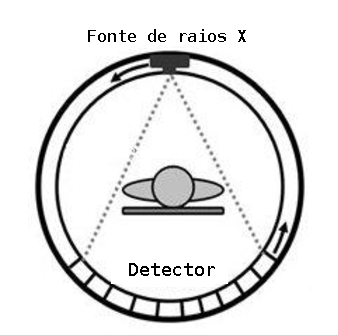
\includegraphics[width=3.5cm]{img/tomografia.pdf}}
	  \column{5cm}{
	    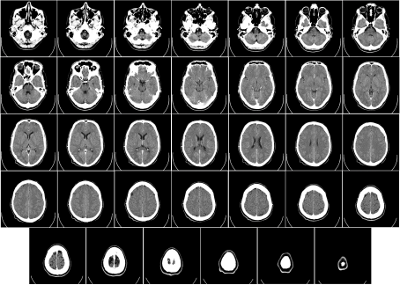
\includegraphics[width=3.5cm]{img/tomografia_2.png}}
	\end{columns}
\end{frame}

\begin{frame}{Exemplos de problemas a serem resolvidos II}
  Modelagem computacional de previsão do tempo (Assimilação de Dados)

	Ciclos de análise: em cada ciclo, as observações sobre o estado atual (e anterior) do sistema são combinados com os resultados de um modelo numérico de previsão do tempo, gerando uma estimativa ao estado atual do sistema (chamada de \emph{análise}. Uma vez que novas observações são feitas, o modelo é atualizado e uma nova previsão (análise futura) pode ser feita a partir do estado atual.
	
	Geração da análise:
	\begin{equation*}
	  \min_x \, \left\{ (x-x_b)^T B^{-1} (x-x_b) + (y-H(x))^TR^{-1}(y-H(x)) \right\}
	\end{equation*}
\end{frame}

\begin{frame}{Como funciona o computador?}
  O computador é uma máquina programável que recebe uma entrada (\emph{input}), armazena e manipula automaticamente dados, e gera uma saída (\emph{output}).
  \begin{center}
		\begin{alertblock}{}
			Um computador executa funções com entrada e saída:
			\begin{center}
				entrada $\rightarrow$ ação $\rightarrow$ saída
			\end{center}
		\end{alertblock}
	\end{center}
\end{frame}

\begin{frame}{Primeiros \emph{computadores}}
  Em 1613, a palavra "computador" aparece pela primeira vez, designando uma \emph{pessoa} que realizasse cálculos.
  
  Os computadores antigos não eram máquinas programáveis, mas serviam a uma função específica. 
  
  Exemplos: ábaco, régua de cálculo, astrolábio, calculadora.
  \vfill
  \begin{columns}
    \column{2cm}
    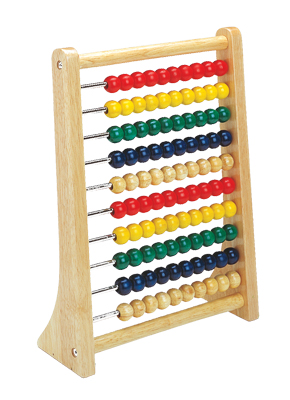
\includegraphics[width=2cm]{img/abaco.jpg}
    \column{2cm}
    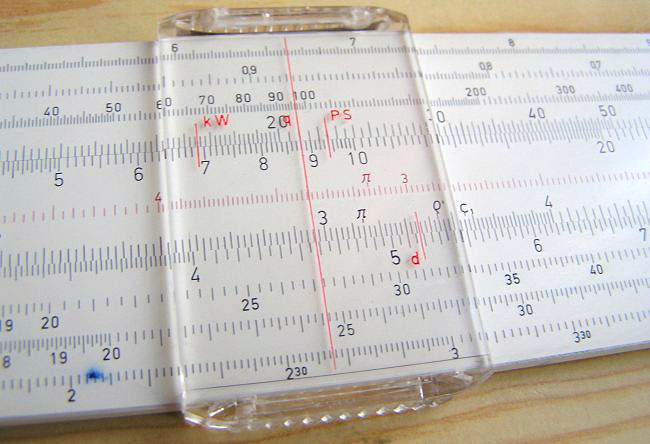
\includegraphics[width=2cm]{img/regua_de_calculo.jpg}
    \column{2cm}
    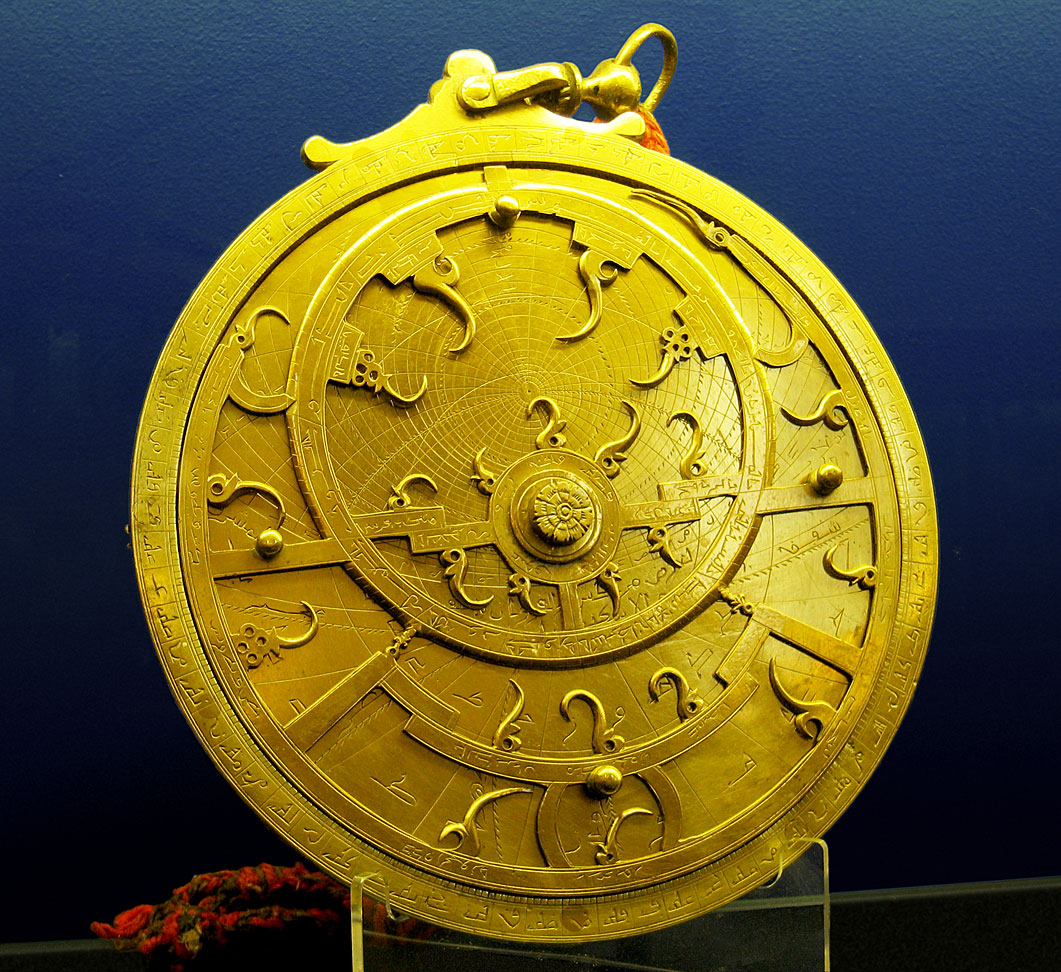
\includegraphics[width=2cm]{img/astrolabio.jpg}
    \column{2cm}
    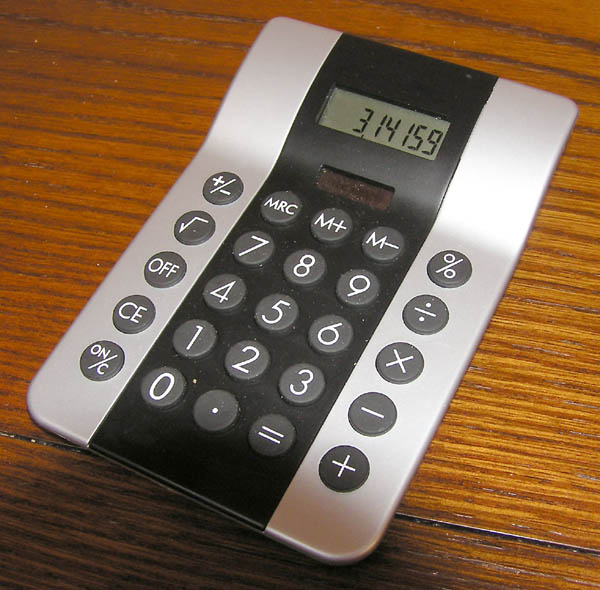
\includegraphics[width=2cm]{img/calculadora.jpg}
  \end{columns}
\end{frame}

\begin{frame}{Computadores programáveis de uso limitado}
  Em 1801, Joseph Marie Jacquard introduziu o uso de cartões perfurados para programar um tear e produzir padrões intrincados de tecido automaticamente.
  \vspace{0.4cm}
  \begin{center}
    \begin{columns}
      \column{5cm}
			\begin{center}
			  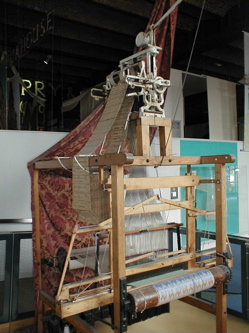
\includegraphics[height=4.5cm]{img/jacquard.jpg}
			\end{center}
      \column{5cm}
			\begin{center}
			  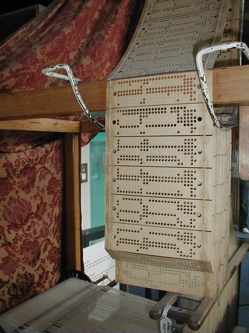
\includegraphics[height=4.5cm]{img/jacquard_cartao.jpg}
			\end{center}
    \end{columns}
  \end{center}
\end{frame}

\begin{frame}{Computadores programáveis de uso geral}
  Em 1837, Charles Babbage imaginou o conceito de um computador mecânico totalmente programável (a \emph{máquina analítica}) - mas não chegou a construi-la.
  \begin{center}
		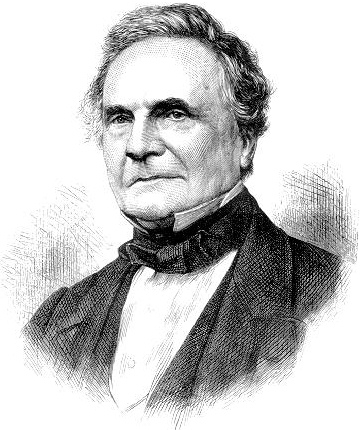
\includegraphics[height=4.5cm]{img/CharlesBabbage.jpg}
	\end{center}
\end{frame}

\begin{frame}{Computadores programáveis de uso geral}
  Ada Augusta Byron King, Condessa de Lovelace, filha do poeta britânico Lord Byron, é reconhecida como a primeira programadora de toda a história. Ela desenvolveu os \emph{algoritmos} que permitiriam à máquina de Babbage computar valores de funções matemáticas, além de publicar uma coleção de notas sobre a máquina analítica.
	\begin{center}
		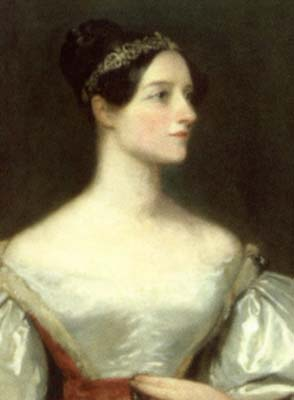
\includegraphics[height=4.5cm]{img/ada.jpeg}
	\end{center}
\end{frame}

\begin{frame}{Estrutura de um computador moderno}
  \begin{center}
    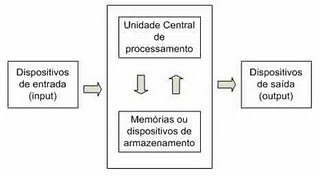
\includegraphics{img/cpu.jpg}
  \end{center}
\end{frame}

\begin{frame}{O que é um algoritmo?}
   \begin{center}
      Um algoritmo é uma sequência \alert{finita} de passos que tem como objetivo realizar alguma tarefa.
   \end{center}

	Exemplo: receita de bolo.
   \begin{itemize}
		\item Entrada: ingredientes, utensílios usados.
		\item Ação: bater, misturar, picar, assar.
		\item Saída: bolo.
	\end{itemize}
\end{frame}

\begin{frame}{Exemplo: Como ferver água (no fogão)?}
	\only<1->{Dada uma cozinha}\only<2->{, com uma pia com torneira e água corrente}\only<3->{, um fogão com pelo menos uma boca}\only<4->{, e uma chaleira ou panela}\only<5->{, faça o seguinte:}
  \only<5->{
    \begin{itemize}}
	\only<5>{\item }
	\only<6->{\item Se encontrar uma chaleira, então use esta chaleira. \\
		Senão, use uma panela.}
  \only<7->{\item Levar a chaleira ou panela até a pia.}
  \only<8->{\item Encher a chaleira ou panela de água.}
  \only<9->{\item Acender uma das bocas do fogão.}
  \only<10->{\item Colocar a chaleira ou panela sobre a boca acesa do fogão.}
  \only<11->{\item Enquanto a água não estiver borbulhando, \\
		continue aguardando.}
  \only<12->{\item Desligue a boca acesa do fogão.}
  \only<5->{
  \end{itemize}}
  \only<13->{A água está fervida dentro da chaleira ou panela.}
\end{frame}

\begin{frame}{Exemplo: Como ferver água (no fogão)?}
  ENTRADA: cozinha, pia, torneira, água corrente, fogão com pelo menos uma boca, chaleira ou panela.\\
  AÇÃO: 
  \begin{itemize}
  \item Se encontrar uma chaleira, então pegue esta chaleira como recipiente. \\
		Senão, pegue uma panela como recipiente.
  \item Levar o recipiente até a pia.
  \item Encher o recipiente de água.
  \item Acender uma das bocas do fogão.
  \item Colocar o recipiente sobre a boca acesa do fogão.
  \item Enquanto a água não estiver borbulhando, \\
		continue aguardando.
  \item Desligue a boca acesa do fogão.
  \end{itemize}
	SAÍDA: recipiente com água fervida.
\end{frame}

\begin{frame}{Exemplo: Como ferver água (no fogão)?}
  ENTRADA: cozinha, pia, torneira, água corrente, fogão com pelo menos uma boca, chaleira ou panela.\\
  AÇÃO: 
  \begin{itemize}
  \item \alert{Se} encontrar uma chaleira, então pegue esta chaleira como recipiente. \\
		\alert{Senão}, pegue uma panela como recipiente.
  \item Levar o recipiente até a pia.
  \item Encher o recipiente de água.
  \item Acender uma das bocas do fogão.
  \item Colocar o recipiente sobre a boca acesa do fogão.
  \item \alert{Enquanto} a água não estiver borbulhando, \\
		\alert{continue} aguardando.
  \item Desligue a boca acesa do fogão.
  \end{itemize}
	SAÍDA: recipiente com água fervida.
\end{frame}

\begin{frame}{Exemplo: Como ferver água (no fogão)?}
  ENTRADA: cozinha, pia, torneira, água corrente, fogão com pelo menos uma boca, chaleira ou panela.\\
  AÇÃO: 
  \begin{itemize}
	\item Se encontrar uma chaleira, então pegue esta chaleira como \textbf{recipiente}. \\
		Senão, pegue uma panela como \textbf{recipiente}.
  \item Levar o \textbf{recipiente} até a pia.
  \item Encher o \textbf{recipiente} de água.
  \item Acender uma das bocas do fogão.
  \item Colocar o \textbf{recipiente} sobre a boca acesa do fogão.
  \item Enquanto a água não estiver borbulhando, \\
		continue aguardando.
  \item Desligue a boca acesa do fogão.
  \end{itemize}
  SAÍDA: recipiente com água fervida.
\end{frame}

\begin{frame}{Exemplo: Como ferver água (no fogão)?}
  ENTRADA: cozinha, pia, torneira, água corrente, fogão com pelo menos uma boca, chaleira ou panela.\\
  AÇÃO: 
  \begin{itemize}
  \item Se existe chaleira, então recipiente \only<1>{\alert{$\leftarrow$}}\only<2>{$\leftarrow$} chaleira. \\
		Senão, recipiente \only<1>{\alert{$\leftarrow$}}\only<2>{$\leftarrow$} panela.
  \item Levar o recipiente até a pia.
  \item Encher o recipiente de água.
  \item \only<1>{Acender uma das bocas do fogão.}
    \only<2>{\alert{Acender} uma das bocas do fogão.}
  \item Colocar o recipiente sobre a boca acesa do fogão.
  \item Enquanto a água não estiver borbulhando, \\
		continue aguardando.
  \item Desligue a boca acesa do fogão.
  \end{itemize}
  SAÍDA: recipiente com água fervida.
\end{frame}

\begin{frame}{O que é uma linguagem de programação?}
	Uma linguagem de programação traduz um algoritmo (sequência de instruções) da linguagem humana para a linguagem da máquina ("0 e 1").
	
	Existem milhares de linguagens de programação.
\end{frame}

\begin{frame}{Módulo: Exemplo em Pseudo-código}
  \begin{center}
	  \begin{itemize}
		\item[] Dado um número $a$
		\item[]
		\item[] Se $a > 0$, então
		  \begin{itemize}
		  \item[] módulo $= a $
		  \end{itemize}
		\item[] Senão
		  \begin{itemize}
		  \item[] módulo $= -a$
		  \end{itemize}
		\item[] Fim Se
	  \end{itemize}
	\end{center}
\end{frame}

\begin{frame}{Exemplo em Python}
  \begin{center}
    \begin{minipage}{0.7\textwidth}
      \lstinputlisting[language=python, title=\texttt{modulo.py}]{listings/modulo.py}
    \end{minipage}
  \end{center}
\end{frame}

\begin{frame}{Exemplo em C}
  \begin{center}
    \begin{minipage}{0.7\textwidth}
      \lstinputlisting[language=c, title=\texttt{modulo.c}]{listings/modulo.c}
    \end{minipage}
	\end{center}
\end{frame}

\begin{frame}{Exemplo em Fortran}
  \begin{center}
    \begin{minipage}{0.7\textwidth}
      \lstinputlisting[language=fortran, title=\texttt{modulo.f}]{listings/modulo.f}
    \end{minipage}
	\end{center}
\end{frame}

\begin{frame}{O que é o MATLAB?}
  \begin{center}
		O MATLAB é uma linguagem computacional e também um ambiente (\emph{framework}) de programação.
		
		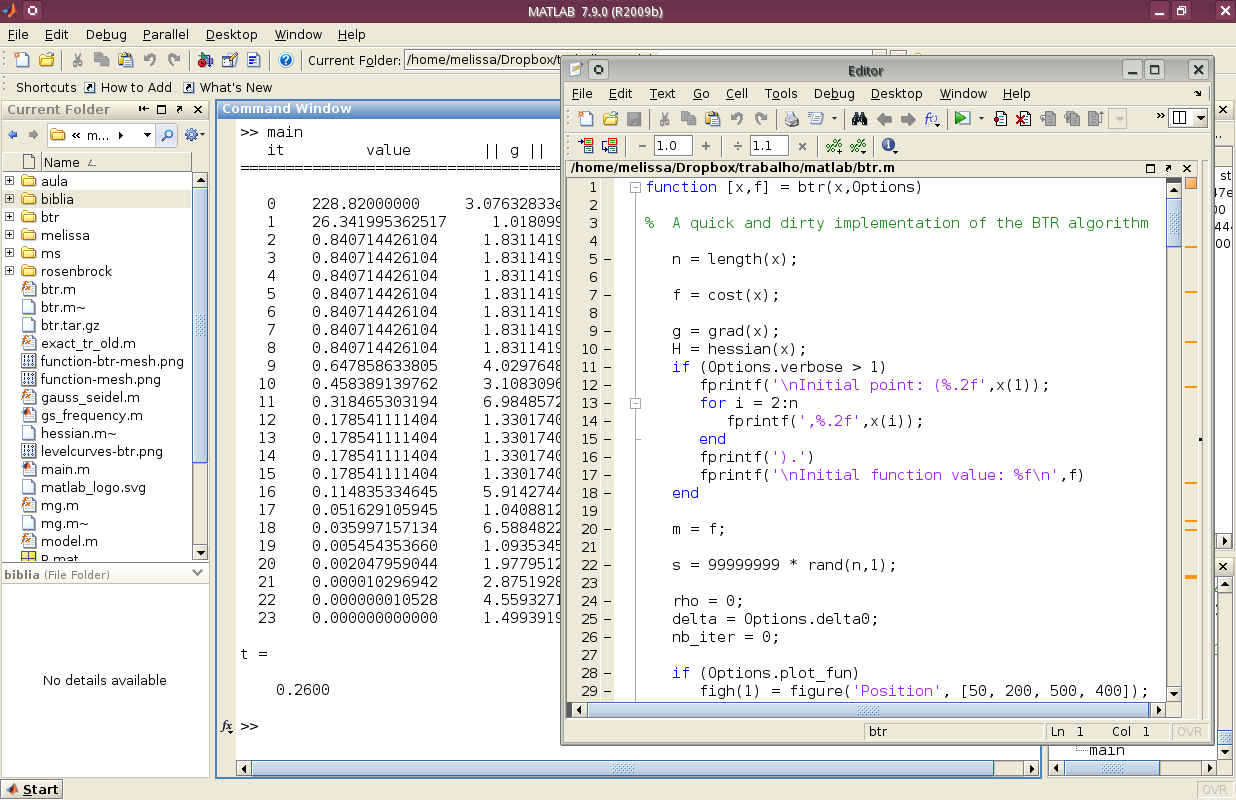
\includegraphics[width=8cm]{img/matlab.png}
  \end{center}
\end{frame}

\begin{frame}{Exemplo de código em MATLAB}
  \begin{center}
    \begin{minipage}{0.7\textwidth}
      \lstinputlisting[title=\texttt{modulo.m}]{listings/modulo.m}
    \end{minipage}
	\end{center}
\end{frame}

\begin{frame}{Octave}
  Também um ambiente de programação, \emph{livre}, gratuito, que suporta a linguagem MATLAB.
  \begin{center}
    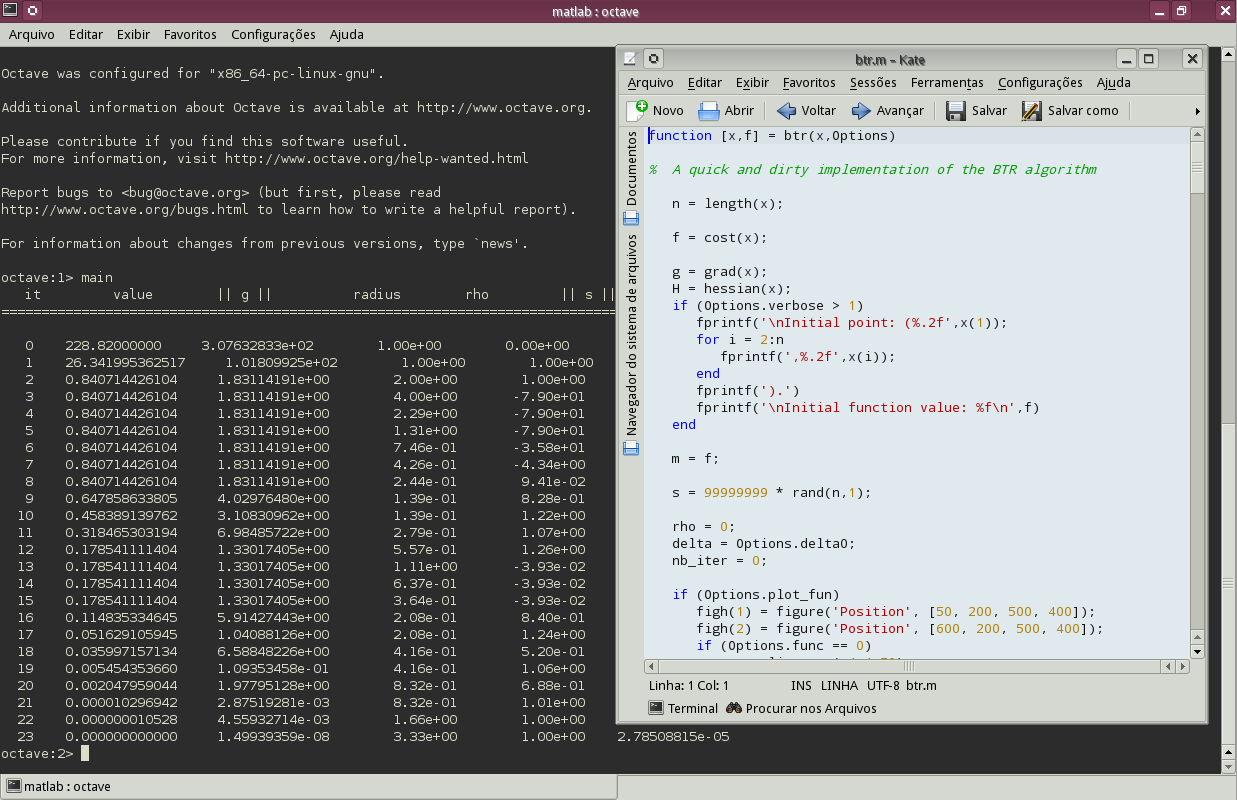
\includegraphics[width=8cm]{img/octave.png}
  \end{center}
\end{frame}

\end{document}
